\documentclass[sigconf]{acmart}
\pdfsuppressptexinfo=-1

\AtBeginDocument{%
  \providecommand\BibTeX{{\normalfont B\kern-0.5em{\scshape i\kern-0.25em b}\kern-0.8em\TeX}}}
% Rights block VERBATIM from ACM's Publication Release Confirmation email of
% 2026-10-14 (copy in ../RIGHTS_BLOCK.tex). "Milan, AA, Italy" is ACM's issued string, kept as issued.
% If the upload checker offers its own block, replace this one wholesale.
\copyrightyear{2026}
\acmYear{2026}
\setcopyright{cc}
\setcctype{by}
\acmConference[ICAIF '26]{7th ACM International Conference on AI in Finance}{November 14--17, 2026}{Milan, AA, Italy}
\acmBooktitle{7th ACM International Conference on AI in Finance (ICAIF '26), November 14--17, 2026, Milan, AA, Italy}
\acmDOI{10.1145/3858063.3858869}
\acmISBN{979-8-4007-3087-0/2026/11}

\usepackage{booktabs}
\usepackage{graphicx}
\usepackage{amsmath}

% GENERATED by code/make_macros.py from data/numbers.json. Do not edit by hand.
% Every quantity in the manuscript resolves through one of these macros.
\newcommand{\ArmCompliance}{100}
\newcommand{\ArmMax}{2.26}
\newcommand{\ArmMedian}{-0.88}
\newcommand{\ArmNullMax}{1.82}
\newcommand{\ArmPermP}{0.14}
\newcommand{\ArmSD}{0.97}
\newcommand{\BestKurt}{6.87}
\newcommand{\BestSkew}{0.93}
\newcommand{\BigCompliance}{99.6}
\newcommand{\BigMax}{1.97}
\newcommand{\BigNullMax}{2.02}
\newcommand{\BigParams}{550B}
\newcommand{\BigPermP}{0.52}
\newcommand{\BigRelease}{2026-06-04}
\newcommand{\BigSD}{0.95}
\newcommand{\BootBetween}{1.30}
\newcommand{\BootFracBestAboveMedian}{100}
\newcommand{\BootGapBestMedianSD}{0.97}
\newcommand{\BootGapBestMedian}{2.69}
\newcommand{\BootRatio}{1.6}
\newcommand{\BootWithin}{0.81}
\newcommand{\CIBest}{[0.64, 4.31]}
\newcommand{\CIDefault}{[-2.38, 1.04]}
\newcommand{\CIMedian}{[-2.24, 1.86]}
\newcommand{\CapControlHigh}{77.7}
\newcommand{\CapControlLow}{75.6}
\newcommand{\CapControlTwoHigh}{96.3}
\newcommand{\CapControlTwoLow}{98.5}
\newcommand{\CapMaxMove}{1.8}
\newcommand{\CapNumCells}{6}
\newcommand{\CapProbeHigh}{256}
\newcommand{\CapProbeN}{300}
\newcommand{\CostBps}{5}
\newcommand{\CostFiveMax}{2.46}
\newcommand{\CostFiveMedian}{-0.24}
\newcommand{\CostFiveSD}{1.01}
\newcommand{\CostLevels}{0, 10 and 25}
\newcommand{\CostTenMax}{2.04}
\newcommand{\CostTenMedian}{-0.84}
\newcommand{\CostTenSD}{1.24}
\newcommand{\CostTwentyfiveMax}{1.58}
\newcommand{\CostTwentyfiveMedian}{-2.36}
\newcommand{\CostTwentyfiveSD}{2.34}
\newcommand{\CostZeroMax}{3.81}
\newcommand{\CostZeroMedian}{0.00}
\newcommand{\CostZeroSD}{0.96}
\newcommand{\DSRfull}{0.072}
\newcommand{\DSRimplied}{0.390}
\newcommand{\DSRliji}{0.335}
\newcommand{\DSRneff}{0.713}
\newcommand{\DSRone}{0.995}
\newcommand{\DefaultPercentileLive}{45}
\newcommand{\DefaultPercentile}{38}
\newcommand{\EmaxFull}{3.84}
\newcommand{\EmaxLiJi}{2.86}
\newcommand{\EmaxMeasured}{2.72}
\newcommand{\EmaxNeff}{1.93}
\newcommand{\EmaxOne}{0.00}
\newcommand{\EtaRatioMedian}{1.04}
\newcommand{\FirstSession}{2025-08-01}
\newcommand{\FracAboveOne}{9}
\newcommand{\FracBelowMinusOne}{27}
\newcommand{\FracEventsPermutable}{99.9}
\newcommand{\FracNeverTrades}{14.8}
\newcommand{\FracPositive}{29}
\newcommand{\GapRaw}{0.26}
\newcommand{\GapStd}{0.06}
\newcommand{\HarnessRange}{5.90}
\newcommand{\HarnessSD}{0.97}
\newcommand{\ICMax}{+0.009}
\newcommand{\ICMean}{-0.012}
\newcommand{\ICMin}{-0.040}
\newcommand{\ICNumConfigs}{18}
\newcommand{\ICNumSig}{1}
\newcommand{\LastSession}{2026-07-30}
\newcommand{\MainParams}{7.6B}
\newcommand{\MaskCorr}{0.68}
\newcommand{\MaskMax}{2.35}
\newcommand{\MaskMedian}{-0.76}
\newcommand{\MaskSD}{0.94}
\newcommand{\MaskShift}{0.054}
\newcommand{\MeanCorr}{0.12}
\newcommand{\MedianEventsPerSession}{11}
\newcommand{\MemConstituents}{502}
\newcommand{\MemFetched}{2026-07-31}
\newcommand{\MemJoiners}{21}
\newcommand{\MemListed}{503}
\newcommand{\MemPreEvents}{48}
\newcommand{\MemPreFirms}{17}
\newcommand{\MemPrePct}{1.6}
\newcommand{\MemRemovals}{22}
\newcommand{\MemRevisionDate}{2026-07-21}
\newcommand{\MemRevision}{1365256480}
\newcommand{\MinDetectAcc}{60}
\newcommand{\ModelEffectRange}{0.59}
\newcommand{\ModelRange}{1.64}
\newcommand{\ModelSD}{0.87}
\newcommand{\NImplied}{160}
\newcommand{\NeffLiJi}{244}
\newcommand{\NeffPct}{0.3}
\newcommand{\Neff}{20}
\newcommand{\NeutralOnlyModel}{5.7}
\newcommand{\NeutralOnlyPostLLM}{7.9}
\newcommand{\NeutralOnlySD}{0.89}
\newcommand{\NullGridSD}{1.10}
\newcommand{\NullMaxMean}{2.72}
\newcommand{\NullMaxPninetyfive}{3.45}
\newcommand{\NullMaxSD}{0.40}
\newcommand{\NumAmendments}{7}
\newcommand{\NumCalls}{53,604}
\newcommand{\NumCodedTotal}{8}
\newcommand{\NumCoded}{7}
\newcommand{\NumConfigs}{7,776}
\newcommand{\NumEventsAvailable}{6,076}
\newcommand{\NumEventsSampled}{3,000}
\newcommand{\NumEvents}{2,978}
\newcommand{\NumLLMConfigs}{18}
\newcommand{\NumLiveConfigs}{6,624}
\newcommand{\NumNeverTrades}{1,152}
\newcommand{\NumPostConfigs}{432}
\newcommand{\NumPredict}{64}
\newcommand{\NumPriceOK}{2,976}
\newcommand{\NumSessions}{250}
\newcommand{\OracleAccHigh}{70}
\newcommand{\OracleAccLow}{55}
\newcommand{\OracleDispDraws}{10}
\newcommand{\OracleFiftyBest}{0.40}
\newcommand{\OracleFiftyP}{0.600}
\newcommand{\OracleFiftyRej}{0}
\newcommand{\OracleFiftyfiveBest}{1.67}
\newcommand{\OracleFiftyfiveP}{0.065}
\newcommand{\OracleFiftyfiveRej}{40}
\newcommand{\OracleFiftytwoBest}{1.25}
\newcommand{\OracleFiftytwoP}{0.187}
\newcommand{\OracleFiftytwoRej}{10}
\newcommand{\OracleSDFiftyfive}{1.00}
\newcommand{\OracleSDRatio}{1.84}
\newcommand{\OracleSDSeventy}{3.30}
\newcommand{\OracleSDSixty}{1.79}
\newcommand{\OracleSeventyBest}{12.21}
\newcommand{\OracleSeventyP}{0.005}
\newcommand{\OracleSeventyRej}{100}
\newcommand{\OracleSixtyBest}{5.52}
\newcommand{\OracleSixtyP}{0.005}
\newcommand{\OracleSixtyRej}{100}
\newcommand{\OracleSpreadFiftyfive}{4.22}
\newcommand{\OracleSpreadSeventy}{14.70}
\newcommand{\OracleSpreadSixty}{7.83}
\newcommand{\PSRBest}{0.995}
\newcommand{\PermPBest}{0.746}
\newcommand{\PermPDefaultDisp}{$>$0.99}
\newcommand{\PermPDefault}{1.000}
\newcommand{\PermReps}{1000}
\newcommand{\PostOnlyRangeMax}{6.31}
\newcommand{\PostOnlyRange}{4.89}
\newcommand{\PostOnlySDMax}{1.24}
\newcommand{\PostOnlySD}{0.94}
\newcommand{\PowerDraws}{10}
\newcommand{\PowerReps}{200}
\newcommand{\ProbePermReps}{300}
\newcommand{\PrudentConfigs}{864}
\newcommand{\PrudentMax}{2.46}
\newcommand{\PrudentMin}{-3.29}
\newcommand{\PrudentRange}{5.75}
\newcommand{\PrudentSD}{0.95}
\newcommand{\RMSCorr}{0.22}
\newcommand{\RobustBest}{2.69}
\newcommand{\RobustIQR}{1.31}
\newcommand{\RobustLags}{5}
\newcommand{\RobustRankCorr}{0.99}
\newcommand{\RobustSDTrimmed}{1.04}
\newcommand{\RobustSD}{1.13}
\newcommand{\SDRatioRealNull}{0.92}
\newcommand{\SDRatio}{1.1}
\newcommand{\SamplePct}{49}
\newcommand{\SampleSeed}{20260731}
\newcommand{\ScaleCompliance}{100}
\newcommand{\ScaleMax}{2.05}
\newcommand{\ScaleMedian}{-0.12}
\newcommand{\ScaleNullMax}{2.06}
\newcommand{\ScaleParams}{36B}
\newcommand{\ScalePermP}{0.48}
\newcommand{\ScaleRelease}{2026-04-16}
\newcommand{\ScaleSD}{1.12}
\newcommand{\SeedCount}{3}
\newcommand{\SeedMedianRange}{0.19}
\newcommand{\SeedTemp}{0.7}
\newcommand{\SharpeBest}{2.46}
\newcommand{\SharpeDefault}{-0.65}
\newcommand{\SharpeIQR}{1.22}
\newcommand{\SharpeMax}{2.46}
\newcommand{\SharpeMedianLive}{-0.51}
\newcommand{\SharpeMedian}{-0.24}
\newcommand{\SharpeMin}{-3.85}
\newcommand{\SharpePfive}{-2.07}
\newcommand{\SharpePninetyfive}{1.32}
\newcommand{\SharpePseventyfive}{0.14}
\newcommand{\SharpePtwentyfive}{-1.08}
\newcommand{\SharpeRange}{6.31}
\newcommand{\SharpeSD}{1.01}
\newcommand{\SplitISBest}{3.73}
\newcommand{\SplitOOSMedian}{0.00}
\newcommand{\SplitOOSPercentile}{72}
\newcommand{\SplitOOSTopTen}{0.40}
\newcommand{\SplitOOSofISBest}{0.53}
\newcommand{\SplitSessions}{125}
\newcommand{\SplitSpearman}{0.15}
\newcommand{\StdIQR}{1.22}
\newcommand{\StdSDLive}{1.08}
\newcommand{\StdSDTrimmed}{0.95}
\newcommand{\TopEigShare}{17}
\newcommand{\TopFactorARange}{0.59}
\newcommand{\TopFactorA}{model}
\newcommand{\TopFactorBRange}{0.50}
\newcommand{\TopFactorB}{signal}
\newcommand{\TopFactorCRange}{0.29}
\newcommand{\TopFactorC}{threshold}
\newcommand{\TriesToOne}{11}
\newcommand{\UnreliableAcc}{55}
\newcommand{\VarShareEntry}{0.3}
\newcommand{\VarShareHold}{1.0}
\newcommand{\VarShareInteractions}{83.3}
\newcommand{\VarShareLLMSide}{8.0}
\newcommand{\VarShareMeanPostLLM}{8.5}
\newcommand{\VarShareModelLive}{7.6}
\newcommand{\VarShareModel}{7.0}
\newcommand{\VarShareNeutral}{0.0}
\newcommand{\VarShareParse}{1.6}
\newcommand{\VarSharePostLLMLive}{9.5}
\newcommand{\VarSharePostLLM}{8.7}
\newcommand{\VarSharePrompt}{0.9}
\newcommand{\VarShareSignal}{4.1}
\newcommand{\VarShareThresh}{1.5}
\newcommand{\VarShareTrimmedModel}{5.9}
\newcommand{\VarShareTrimmedPostLLM}{11.8}
\newcommand{\VarShareTrunc}{0.1}
\newcommand{\VarShareVolModel}{3.4}
\newcommand{\VarShareVolPostLLM}{33.3}
\newcommand{\VarShareWeight}{0.2}

% Public artifact link. consistency.py checks that it is a live https URL.
\newcommand{\ArtifactURL}{\url{https://github.com/s1mar/grid-is-the-alpha}}

\begin{document}

\title{The Grid Is the Alpha: Measuring Effective Multiplicity and
Permutation Nulls in LLM Event-Driven Trading}

\author{Simarjot Khanna}
\orcid{0009-0009-4827-9884}
\affiliation{%
  \institution{Independent Researcher}
  \country{Canada}
}
\email{simarkhanna76@gmail.com}

\begin{abstract}
Papers that report trading performance for large language models describe one pipeline: one prompt,
one way of reading the model's answer, one holding period, one entry rule. Behind that one number is
a search whose size is rarely reported. We measure the effective multiplicity of one such search and
benchmark it against a permutation null that any paper can run on the grid it has already computed.
Over \NumEvents{} SEC Form 8-K filings from \FirstSession{} to \LastSession{}, a window opening more
than ten months after the most recent model in our grid was released, we build one event-driven
equity pipeline over three open-weight models under 8 billion parameters and evaluate a
pre-registered grid of \NumConfigs{} configurations differing only in choices papers rarely report. Annualised Sharpe runs from \SharpeMin{} to \SharpeMax{}, standard
deviation \SharpeSD{}; with model, prompt and truncation all fixed, the \NumPostConfigs{}
configurations reachable \emph{after} the model has spoken still span \PostOnlyRange{} on average.
No family of choices is the culprit: on a descriptive partition, \VarShareInteractions{}\% of the
variance sits in interactions rather than in any main effect. The configurations are highly correlated, so the effective number of
independent
trials is \Neff{} by the cheapest estimator and \NImplied{} by measurement, against a nominal
\NumConfigs{}, and the deflated Sharpe ratio of the best configuration moves from \DSRone{} through
\DSRimplied{} to \DSRfull{} depending on which count is assumed. We
replace that assumption with a measurement: a within-session permutation benchmark, run over the
identical grid, gives a best-of-grid Sharpe of \NullMaxMean{} when the model's scores are permuted
among the filings of each session, against \SharpeBest{} for the real pipeline
($p=\PermPBest{}$). In this study, the grid run on permuted scores reaches a higher best-of-grid
Sharpe, on average, than the real pipeline. We close with a reporting protocol built on the
same two instruments.
\end{abstract}

\begin{CCSXML}
<ccs2012>
<concept><concept_id>10010405.10010481</concept_id>
<concept_desc>Applied computing~Economics</concept_desc><concept_significance>500</concept_significance></concept>
<concept><concept_id>10010147.10010257</concept_id>
<concept_desc>Computing methodologies~Machine learning</concept_desc><concept_significance>300</concept_significance></concept>
</ccs2012>
\end{CCSXML}
\ccsdesc[500]{Applied computing~Economics}
\ccsdesc[300]{Computing methodologies~Machine learning}

\keywords{large language models, backtest overfitting, multiple testing, deflated Sharpe ratio,
event-driven trading, reproducibility}

\maketitle

\section{Introduction}

A large and fast-growing literature reports that language models can trade. The reported artifact is
almost always a single number attached to a single pipeline: this prompt, this model, this rule for
turning the model's text into a position, this holding period. The pipeline has many more moving
parts than that, and most of them are never described.

This paper measures what those parts are worth. We build one event-driven equity pipeline over SEC
Form 8-K filings, and instead of reporting its Sharpe ratio we report the distribution of Sharpe
ratios over a pre-registered grid of \NumConfigs{} configurations that differ only in choices that
published pipelines leave unstated. The grid is deliberately not a search for alpha. It is an
enumeration of the freedom a researcher has after deciding to do the study at all.

The concern is not new in finance. Bailey and L\'opez de Prado \cite{bailey2014deflated} argue that
a backtest whose author has not controlled for the extent of the search is uninformative regardless
of how good it looks, and give the deflated Sharpe ratio to correct for it. Harvey, Liu and Zhu
\cite{harvey2016cross} raise the significance bar for factor discovery for the same reason. Menkveld
et al.~\cite{menkveld2024nonstandard} let 164 teams test the same hypotheses on the same data and
find the resulting dispersion sizeable, and underestimated by the researchers themselves. In machine learning the same fragility is documented for prompts: formatting alone moves
benchmark accuracy by up to 76 accuracy points on one model \cite{sclar2024quantifying}, and the
order of few-shot examples separates near state of the art from random guessing
\cite{lu2022fantastically}.

What has not been done is to measure the two together in a trading pipeline. A position paper by Ye
et al.~\cite{ye2026alpha} argues that public evidence cannot yet separate robust predictive ability
from confounders such as short-window Sharpe uncertainty and narrative fitting, proposes a minimum
reporting protocol, and reports no experiments. This paper supplies measurement where that position
supplies standards, and the number needed to apply the existing correction: the effective number of
trials.

\medskip\noindent\textbf{Contributions.}
\begin{enumerate}\itemsep1pt
\item \textbf{An effective trial count and a permutation benchmark.} The grid is nowhere near
      \NumConfigs{} independent trials, and the estimator matters: the cheap participation ratio
      gives \Neff{}, the Li and Ji count gives \NeffLiJi{}, and the permutation benchmark says the
      grid behaves like \NImplied{}. Permuting the model's outputs among the filings of the same
      session and re-running the identical grid gives the distribution of best-of-grid Sharpe when
      those outputs carry no within-session information, and the real pipeline does not exceed it
      (Section~\ref{sec:multiplicity}).
\item \textbf{The correction depends on a number papers rarely report.} We evaluate the expected-maximum
      formula behind the deflated Sharpe ratio at four assumed trial counts and at the count the
      permutation implies, and on this grid the spectral count that is easiest to compute is the
      one that under-corrects most (Section~\ref{sec:multiplicity}).
\item \textbf{A measured dispersion.} Over one fixed event set, one universe and one window,
      annualised Sharpe ranges from \SharpeMin{} to \SharpeMax{} across \NumConfigs{} configurations
      that a reader of any single paper could not tell apart. With the model, prompt and truncation
      held fixed, the post-LLM choices alone span \PostOnlyRange{} (Section~\ref{sec:dispersion}).
\item \textbf{No scapegoat, and the reason.} The pre-registered comparison holds, narrowly: the
      seven post-LLM choices account for \VarSharePostLLM{}\% of the variance against
      \VarShareModel{}\% for the model, which is the largest \emph{single} main effect, while
      \VarShareInteractions{}\% of the variance sits in interactions, so neither family can be
      blamed on this evidence (Section~\ref{sec:variance}).
\item \textbf{A protocol and an estimator} that a paper can run on any grid it has already computed,
      with the artifact released (Section~\ref{sec:protocol}).
\end{enumerate}

The grid, the sample, the primary statistics and the falsification condition were pre-registered
before any return was computed, and the pre-registration ships with the artifact alongside a
declared count of \NumAmendments{} amendments. The robustness arms in Section~\ref{sec:probes} are
not covered by that claim: they were added after the pre-registered analysis was complete, in
response to review, and they are declared as such rather than presented as planned.

\section{Related work}

\textbf{Backtest overfitting and multiple testing.} Selection over trials inflates the selected
Sharpe ratio, and the inflation grows with the number of trials \cite{bailey2014pseudo}. The
deflated Sharpe ratio \cite{bailey2014deflated} corrects for this given the number of independent
trials $N$, the dispersion of the trial Sharpe ratios, and the higher moments of the selected
strategy's returns; the probabilistic Sharpe ratio \cite{bailey2012sharpe} is its single-trial
ancestor. White's reality check \cite{white2000reality} bootstraps the distribution of the maximum
statistic across strategies. All of this machinery was built for parameter grids over price-based
rules. We apply it where the trials are not strategies but implementation choices, most of which the
researcher does not think of as choices.

\textbf{Undisclosed flexibility.} Simmons et al.~\cite{simmons2011false} showed that flexibility in
analysis, undisclosed, is sufficient to make almost anything significant. Menkveld
et al.~\cite{menkveld2024nonstandard} measured the finance version across 164 teams. Their design
cannot attribute the dispersion to a particular decision, because the teams differ in every decision
at once. Ours can, because the decisions are enumerated rather than delegated.

\textbf{LLMs that trade.} Lopez-Lira and Tang \cite{lopezlira2023chatgpt} score news headlines and
report daily long-short returns. A line of agentic systems followed
\cite{yu2023finmem,zhang2024finagent,yu2024fincon,xiao2024tradingagents,papadakis2025atlas}. Li
et al.~\cite{li2025finsaber} audit this literature by varying the market: longer horizons and
different regimes, with the pipeline held fixed. We do the orthogonal audit, holding the market
fixed and varying the pipeline. Glasserman and Lin \cite{glasserman2023assessing} study look-ahead
contamination and find that masking company identifiers changes measured performance, which is why
we place our entire sample after the release of every model in the pre-registered grid rather than
argue about it, and why we also run an entity-masked arm.

\textbf{Reporting practice.} Table~\ref{tab:coding} records what a reader can recover from
\NumCodedTotal{} recent pipelines, \NumCoded{} coded from machine-readable full text. It is a
convenience sample coded by one author: it illustrates practice, it does not survey it. The point is
not carelessness, since Lopez-Lira and Tang \cite{lopezlira2023chatgpt} give their prompt, their rebalancing
rule, their exact entry rule and four cost levels. It is that the union of what the sample reports is small, and none
of the \NumCoded{} we could code reports a sensitivity analysis over implementation choices rather
than components or the market.

\begin{table}[t]
\centering
\caption{What \NumCodedTotal{} recent LLM trading pipelines report. \checkmark{} means a sentence
stating the item was located in the paper's full text; a blank means it was not. \emph{Sensitivity}
means a robustness analysis over implementation choices; $\dagger$ marks a paper that ablates
\emph{components} instead, which is a different thing and is why the text says no paper we could
code reports the former.}
\label{tab:coding}
\small
% GENERATED by code/make_macros.py from data/paper_coding.json.
\begin{tabular}{lccccc}
\toprule
 & prompt & holding & entry & sensi- & costs \\
 & text & period & timing & tivity & \\
\midrule
Lopez-Lira and Tang \cite{lopezlira2023chatgpt} & \checkmark & \checkmark & \checkmark &  & \checkmark \\
FinMem \cite{yu2023finmem} & \multicolumn{5}{c}{\textit{full text not machine-readable}} \\
FinAgent \cite{zhang2024finagent} &  &  &  & $\dagger$ &  \\
FinCon \cite{yu2024fincon} &  & \checkmark &  & $\dagger$ &  \\
TradingAgents \cite{xiao2024tradingagents} &  &  &  &  &  \\
FINSABER \cite{li2025finsaber} &  &  &  &  & \checkmark \\
ATLAS \cite{papadakis2025atlas} &  & \checkmark &  &  &  \\
Huang et al. \cite{huang2026hypotheses} &  & \checkmark & \checkmark &  & \checkmark
\\
\bottomrule
\end{tabular}

\end{table}

\section{The pipeline}
\label{sec:pipeline}

\subsection{Data}

The universe is the \textbf{S\&P 500} constituent list on Wikipedia, retrieved on \MemFetched{}, the
day after the last session. The page was then at revision \MemRevision{}, dated \MemRevisionDate{}.
It lists \MemListed{} constituents. One row, for Cboe Global Markets, uses a different ticker format
and was not parsed, so the universe holds \MemConstituents{} names. The event pool is every
Form 8-K filed in the window by one of those names, \NumEventsAvailable{} filings after collapsing
dual-class duplicates; 8-K filings are the SEC's current-report mechanism and are known to move
prices \cite{lerman2010new}. We score a seed-fixed random subsample of \NumEventsSampled{},
\SamplePct{}\% of the pool, because the full factorial did not fit the available compute; this is a
declared amendment and the draw ships in the artifact. Of those, \NumEvents{} filings leave room for
the longest holding period, and \NumPriceOK{} of these have every price a position needs; no
configuration takes a position in the other two. For each filing we
retrieve the primary document and its EX-99 exhibits from EDGAR and strip the markup. Prices are
daily open, close and split- and dividend-adjusted close; the benchmark is SPY.

Two properties of this source matter. First, every filing carries an exact acceptance timestamp, so
whether a configuration could have traded on it is a fact rather than an assumption. Second, the
window opens more than ten months after the most recent of the three scoring models in the grid was
publicly released. A model cannot have been trained on text published after its own release, so this
is a hard bound whether or not a cutoff is documented; the one model of the three whose card states
a training-data cutoff gives October 2023. No configuration \emph{in the grid} can therefore owe its
performance to a memorised outcome, which is a stronger position than the usual argument about
contamination \cite{glasserman2023assessing} and it costs nothing, because the data source is
current. The bound does not extend to the two post hoc scale arms added in Section~\ref{sec:probes},
whose models were released mid-window; that exception is stated where the arms are reported and
again in Threats.

\subsection{Fixed elements}

Four things are held fixed, so that none of them is a \emph{factor} in the grid. They are not
therefore inert: a constant applied to configurations that differ in turnover, exposure or holding
period can still change the spread between them, and Section~\ref{sec:probes} measures exactly that
for the cost assumption. (i) An event is tradable only in the first regular session that opens
strictly after its acceptance timestamp, converted to Eastern time. (ii) Transaction costs are
\CostBps{} basis points per side on traded notional, in the range used by comparable studies
\cite{lopezlira2023chatgpt,huang2026hypotheses}. (iii) Decoding is greedy with a fixed seed, so the
reported dispersion is design, not sampling noise. (iv) Filing text is assembled as item codes,
then exhibits, then the primary document, chosen so truncation does not hand every model an earnings
8-K's cover page pointing at Exhibit 99.1. We did not measure alternative orderings.

\subsection{The grid}

The factors are listed in Table~\ref{tab:grid}. Three are LLM-side, and each combination of their
levels costs a separate inference pass; seven are post-LLM and re-use the same raw model output, which is why a grid of this size is
affordable at all. We call these choices \emph{undisclosed} rather than meaningless. A five-day hold
is not a one-day hold. The claim is narrower and checkable: no theory in this literature determines
any of these levels, and Table~\ref{tab:coding} shows that most of them go unreported.

\begin{table}[t]
\centering
\caption{The pre-registered factor grid: $\NumLLMConfigs{} \times \NumPostConfigs{} = \mbox{\mdseries\NumConfigs{}}$
configurations, each evaluated on the identical events, prices and window.}
\label{tab:grid}
\small
\begin{tabular}{llc}
\toprule
factor & levels & $\vert\cdot\vert$ \\
\midrule
\multicolumn{3}{l}{\textit{LLM-side (one inference pass per combination of levels)}}\\
model & Qwen2.5-7B, Mistral-7B-v0.2, Phi-3-mini & 3 \\
prompt & analyst probability; label with & 3 \\
       & confidence; JSON with a no-view option & \\
truncation & 1200, 4000 characters & 2 \\
\midrule
\multicolumn{3}{l}{\textit{post-LLM (no new inference per level: the same raw output is re-read)}}\\
parsing & strict (drop non-conforming answers), & 2 \\
        & lenient (salvage, else neutral) & \\
signal & level, cross-sectional rank, & 3 \\
       & expanding per-ticker demeaning & \\
threshold & 0.00, 0.10, 0.20 deadband & 3 \\
holding & 1, 3, 5 sessions & 3 \\
entry & next open, next close & 2 \\
weighting & equal, proportional to $\vert$signal$\vert$ & 2 \\
neutralisation & none, subtract net exposure $\times$ SPY & 2 \\
\bottomrule
\end{tabular}
\end{table}

\begin{table}[t]
\centering
\caption{Percentage of filings for which the model answered in the format the prompt asked for, so
that a strict parser accepts it. A cell at or near zero means that under a strict parser that
model-prompt combination has almost no tradable events. Whether it trades is therefore joint: the same
output is usable under a lenient parser and unusable under a strict one.}
\label{tab:compliance}
\small
% GENERATED by code/make_macros.py. Do not edit by hand.
\begin{tabular}{lccc}
\toprule
 & P1 probability & P2 label & P3 JSON \\
\midrule
Qwen2.5-7B & 100.00 & 99.98 & 99.98 \\
Mistral-7B-v0.2 & 0.00 & 0.00 & 74.01 \\
Phi-3-mini & 0.15 & 92.11 & 4.35 \\
\bottomrule
\end{tabular}

\end{table}

\section{Statistical framework}
\label{sec:stats}

\textbf{Effective trials.} The configurations are not independent: they share events, prices and, in
most cases, scores. Let $Z$ be the $N \times T$ matrix of standardised daily configuration returns
and $C = ZZ^\top/T$ its correlation matrix, whose eigenvalues $\lambda_i$ sum to $N$. We take the
participation ratio
\begin{equation}
N_{\mathrm{eff}} = \Big(\textstyle\sum_i \lambda_i\Big)^2 \Big/ \textstyle\sum_i \lambda_i^2
= N^2 \Big/ \textstyle\sum_{ij} C_{ij}^2 ,
\label{eq:neff}
\end{equation}
which needs no eigendecomposition, and report the eigenvalue count of Li and Ji
\cite{li2005adjusting} as a second estimate. Because $\mathrm{rank}(Z) \le T$, all nonzero
eigenvalues are obtained from a $T \times T$ matrix.

\textbf{Deflated Sharpe.} With $\widehat{SR}$ the per-observation Sharpe of the selected
configuration, $V$ the variance of the trial Sharpe ratios, $\gamma$ the Euler-Mascheroni constant
and $Z(\cdot)$ the standard normal CDF, Bailey and L\'opez de Prado's expected maximum over $N$
independent trials is
\begin{equation}
\mathbb{E}\big[\max \widehat{SR}\big] \approx
\sqrt{V}\Big((1-\gamma)Z^{-1}\big[1-\tfrac{1}{N}\big] + \gamma Z^{-1}\big[1-\tfrac{1}{Ne}\big]\Big),
\label{eq:emax}
\end{equation}
and the deflated Sharpe ratio is the probability that the selected Sharpe exceeds that threshold,
adjusted for skewness and kurtosis \cite{bailey2014deflated}. The open question in any application
is what to use for $N$.

\textbf{A permutation benchmark.} We replace that assumption with a measurement. In each of
\PermReps{} replications the assignment of model outputs to filings is permuted within each entry
session, destroying the link between a filing and its score while preserving the daily score
distribution, the number of positions per day and the correlation structure across configurations.
The full grid is re-evaluated each replication.

Being precise about what this tests matters more than the arithmetic. The null it enforces is that
the model's outputs are exchangeable \emph{within a session}, that is, that they carry no
information about which of that session's filings they belong to. It is not the general claim that
the model contributes nothing: because session-level score distributions are preserved, any
market-timing content survives permutation untested, and model outputs could still vary
systematically with issuer or filing type. Nor is it exact in the combinatorial sense; with
\PermReps{} sampled reassignments it is a Monte Carlo permutation distribution. What it does give is
a benchmark computed on the same events, the same prices and the same grid, and it is the negative
half of a two-sided control for the harness, whose positive half is the oracle sweep in
Section~\ref{sec:multiplicity}: a pipeline that reports a high number here is measuring its own
grid.

\textbf{Intervals.} Confidence intervals on individual configurations use a stationary bootstrap
\cite{politis1994stationary} with mean block length five sessions. To separate the spread across
configurations from the sampling error of any one of them, sessions are resampled once per
replication and every configuration is re-evaluated on the same resampled sessions, so the sampling
error they share cancels and what remains is the error of the differences between them.

\textbf{Configurations that never trade.} A configuration can be well defined and still hold nothing:
a strict parser rejecting every answer from a model-prompt cell leaves it with no positions and a
Sharpe of $0/0$. We record those at zero, the limit of a strategy that holds nothing, keep them
because a researcher choosing that configuration would face exactly this outcome, and report how
many.

\section{Results}
\label{sec:results}

\subsection{Dispersion}
\label{sec:dispersion}

Across \NumConfigs{} configurations of a single pipeline, evaluated on identical events and prices,
annualised Sharpe runs from \SharpeMin{} to \SharpeMax{}, with a standard deviation of \SharpeSD{}
and an interquartile range of \SharpeIQR{} (Figure~\ref{fig:dispersion}). Most configurations lose money: \FracPositive{}\% are profitable before any deflation and
\FracAboveOne{}\% clear a Sharpe of one, so a researcher drawing settings independently until one
did would expect to succeed in about \TriesToOne{} attempts. That count assumes independent draws,
which Section~\ref{sec:multiplicity} shows the grid does not supply; it is the number a researcher
who believed the settings were independent would predict. \FracNeverTrades{}\% of the grid never
trades, because a strict parser can reject every answer a given model gives to a given prompt
(Table~\ref{tab:compliance}); those are recorded at zero, which is above the grid median, so every
percentile here is over the whole grid and shifts if they are dropped. Excluding the never-trading
configurations the median is \SharpeMedianLive{} and the default sits at the
\DefaultPercentileLive{}th percentile rather than the \DefaultPercentile{}th; the spread widens to
\StdSDLive{} from \SharpeSD{}, and the range, the best configuration and its permutation p-value
are unchanged, because both extremes are configurations that trade.

The three configurations in Table~\ref{tab:refconfigs} are the ones a paper might report: our
default returns \SharpeDefault{} at the \DefaultPercentile{}th percentile, the grid median
\SharpeMedian{}, the best \SharpeBest{}. The
default is our own choice of a plausible unexamined setting, not a measured modal practice:
Table~\ref{tab:coding} records what papers \emph{disclose}, which is not enough to identify what
they chose. The bootstrap intervals overlap, which is the point: these are not three strategies with
different merits, they are three trading configurations built from one event set and one archive of
model outputs, and nothing in any of the coded papers would let a reader tell which one was used.

The sharpest form needs no comparison between models. Holding the model, prompt and truncation fixed
and letting only the \NumPostConfigs{} post-LLM configurations vary, the Sharpe ratios inside one
such cell have a standard deviation of \PostOnlySD{} and span \PostOnlyRange{} on average, up to
\PostOnlyRangeMax{} in the widest. Every number in that range describes the same
model reading the same filings.

The natural objection is that a Sharpe ratio over \NumSessions{} sessions is noisy enough to produce
this spread on its own. Resampling sessions and re-evaluating every configuration on the same
resample leaves a between-configuration spread of \BootBetween{} against a within-configuration
sampling standard deviation of \BootWithin{}, a ratio of \BootRatio{}: sampling error is a real
component of what any single reported Sharpe ratio means, and it is the smaller one. The gap between
the best and the median configuration averages \BootGapBestMedian{} (sd \BootGapBestMedianSD{})
across resamples, and the best stays above the median in \BootFracBestAboveMedian{}\% of them.

\begin{figure}[t]
\centering
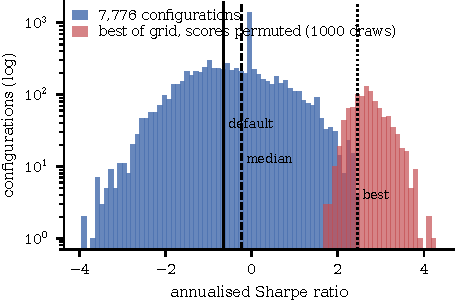
\includegraphics[width=0.58\columnwidth]{fig_dispersion.pdf}
\Description{Two overlaid histograms of annualised Sharpe ratio, with counts on a logarithmic axis. The blue histogram covers the \NumConfigs{} configurations, from \SharpeMin{} to
\SharpeMax{}, with vertical lines at the default configuration, the median and the best
configuration. The red histogram shows the best-of-grid Sharpe ratio in each of \PermReps{}
permutation draws. It sits at the right end of the blue histogram, and most of its draws lie beyond
the line of the best configuration.}
\caption{Every configuration is the same pipeline on the same events, prices and window. The red
distribution is the best-of-grid Sharpe when the model's outputs are permuted among the filings of
the same session, so that they carry no within-session information.}
\label{fig:dispersion}
\end{figure}

\begin{table}[t]
\centering
\caption{Three ways of reporting the same pipeline, and what the grid produces on permuted scores. The last row
is the benchmark, not a fourth way of reporting: the mean best-of-grid annualised Sharpe when scores
are permuted among filings of the same session, and it is \emph{higher} than the grid maximum above
it. The intervals are stationary-bootstrap intervals for each configuration on its own, unadjusted
for the search that selected it; the permutation p-values in Section~\ref{sec:multiplicity} account
for that search.}
\label{tab:refconfigs}
\small
\begin{tabular}{lrl}
\toprule
what is reported & Sharpe & 95\% CI \\
\midrule
our default configuration           & \SharpeDefault{} & \CIDefault{} \\
the grid median                     & \SharpeMedian{}  & \CIMedian{} \\
the grid maximum                    & \SharpeBest{}    & \CIBest{} \\
\midrule
best of grid, scores permuted       & \NullMaxMean{}   & \\
\bottomrule
\end{tabular}
\end{table}

\subsection{Where the variance comes from}
\label{sec:variance}

A balanced sum-of-squares partition splits the variance of Sharpe across the grid into marginal
main effects. The configurations share events, prices and scores, so these shares are descriptive
accounting rather than a causal decomposition over independent cells, and they are computed over
the whole grid, including the never-trading configurations at zero; excluding those leaves the
ordering intact at \VarSharePostLLMLive{}\% against \VarShareModelLive{}\%. The pre-registered comparison
holds: the seven post-LLM choices account for \VarSharePostLLM{}\% of the variance and the language
model for \VarShareModel{}\%. That is seven marginal shares against one, with most of the variance
in neither, so it settles less than it appears to. The largest \emph{single} main effect is
\TopFactorA{}, which moves
mean Sharpe across its levels by \TopFactorARange{}, and the runner-up is \TopFactorB{} at
\TopFactorBRange{}. Stated without the analysis of variance, whose observations are not independent
draws: swapping the language model with every other choice held fixed moves Sharpe by \ModelSD{} on
average, and re-deciding the pipeline around a fixed model moves it by \HarnessSD{}, a ratio of only
\SDRatio{}.

The conclusion is not that one family of choices is to blame. It is that \VarShareInteractions{}\%
of the variance sits in interactions rather than in any main effect, so on this evidence no family
can be. Table~\ref{tab:compliance} makes one such interaction concrete, though it does not establish
that this one is the largest. Qwen2.5-7B answers all three prompts in the requested format on
essentially every filing; the two smaller models each comply with a \emph{different} single prompt
and are at or near zero on the other two. Under a
strict parser, ``which model'' and ``how strictly do you parse the answer'' are therefore not two
questions but one, and most papers disclose neither. A one-factor-at-a-time
sensitivity analysis, which is what a reviewer would normally ask for, cannot see this at all.

One qualification the decomposition itself supplies. Run the same partition on the two components of
the Sharpe ratio separately: the post-LLM choices carry \VarShareMeanPostLLM{}\% of the variance of
mean daily return but \VarShareVolPostLLM{}\% of the variance of daily volatility. Much of what they
do is rescale risk rather than change the return earned, which is a real effect on a reported
statistic and a smaller effect on a portfolio someone volatility-targets first.

Two checks that the ranking is not an artifact of how we drew the grid. Dropping the most aggressive
level of the two factors a reviewer would name first, the 0.20 deadband and the five-day hold,
leaves the post-LLM share at \VarShareTrimmedPostLLM{}\% against \VarShareTrimmedModel{}\%, a wider
margin than in the full grid. And because the models are optimistic on average, a configuration
that neither demeans nor neutralises is partly holding the market; inside the market-neutral half
alone the spread is still \NeutralOnlySD{} and the post-LLM share \NeutralOnlyPostLLM{}\% against
\NeutralOnlyModel{}\%.

\subsection{Multiplicity}
\label{sec:multiplicity}

The \NumConfigs{} configurations are not \NumConfigs{} trials. Their daily returns have a mean
pairwise correlation of \MeanCorr{} and a root-mean-square correlation of \RMSCorr{}, the quantity
equation~\eqref{eq:neff} responds to since it squares $C_{ij}$ and is blind to sign; the leading
eigenvalue carries \TopEigShare{}\% of the total,
and equation~\eqref{eq:neff} gives $N_{\mathrm{eff}} = \Neff{}$, which is \NeffPct{}\% of the
nominal grid; the Li and Ji count gives \NeffLiJi{}. A researcher who treats the reported
configuration as a single trial and one who applies a Bonferroni count over the whole grid are
wrong in opposite directions, the Bonferroni count by more than two orders of magnitude and the
single-trial count by more than one.

Table~\ref{tab:multiplicity} shows what that choice is worth. The deflated Sharpe ratio of the best
configuration is \DSRone{} if the grid is ignored, \DSRneff{} at $N_{\mathrm{eff}}$, \DSRliji{} at
the Li and Ji count and \DSRfull{} at the nominal grid size. The same backtest is overwhelming
evidence or none at all, depending on a number papers rarely report. Equation~\eqref{eq:emax} is
evaluated throughout at a mean trial Sharpe of zero, the null the deflated Sharpe ratio is defined
against, so the $N=1$ row is zero by construction.

The permutation null settles it without any of those assumptions. Over \PermReps{} replications
permuting the model's outputs among filings of the same session, the best-of-grid Sharpe averages
\NullMaxMean{} (sd \NullMaxSD{}, 95th percentile \NullMaxPninetyfive{}) against \SharpeBest{} for
the real pipeline, a p-value of \PermPBest{}; the default configuration gives \PermPDefaultDisp{}.
The median session carries \MedianEventsPerSession{} events and \FracEventsPermutable{}\% sit in
sessions with at least one other, so the reassignment is far from degenerate and the null is
conservative only to the small extent that it is not. The null grid is also slightly wider,
\NullGridSD{} against \SharpeSD{}, which raises its maximum: standardising each grid by its own
spread narrows the gap from \GapRaw{} to \GapStd{}, so part of what the benchmark shows is
dispersion rather than level.

\textbf{A benchmark that rejects nothing proves nothing.} A permutation test is a negative control,
and on its own it cannot separate ``these models carry no within-session information'' from ``this
pipeline could not have detected information if it were there''. So we built the positive half.
A synthetic score of known directional accuracy, costing no model inference, is pushed through the
identical grid and the identical benchmark, here at \PowerReps{} replications rather than the
\PermReps{} used above, so its p-values are bounded below by $1/(\PowerReps{}+1)$. A single
synthetic dataset would establish only that some alternative is detectable, which is a sensitivity
check and not an estimate of power, so we draw \PowerDraws{} independent oracles at each accuracy
and report the share of them the benchmark rejects at the 5\% level. At 50\% it rejects
\OracleFiftyRej{}\% of draws (median best \OracleFiftyBest{}, median $p=\OracleFiftyP{}$), which is
the negative control behaving correctly, and at 52\% it rejects \OracleFiftytwoRej{}\%. At
\UnreliableAcc{}\% it rejects \OracleFiftyfiveRej{}\% of draws with a median $p$ of
\OracleFiftyfiveP{}: an edge of that size is found less often than not, and a single draw at that
accuracy can produce a significant result or an insignificant one. At 60\% it rejects
\OracleSixtyRej{}\% of draws and at 70\% \OracleSeventyRej{}\%, with median p-values at the floor
that replication count allows. So \MinDetectAcc{}\% is the lowest level we tested that was rejected
in all \PowerDraws{} draws, and \UnreliableAcc{}\% is a level detected inconsistently, in
\OracleFiftyfiveRej{}\% of draws, rather than a detection.
Every dispersion figure we report is otherwise measured on scores with no detectable signal, so the
oracle also settles whether the spread survives when signal is present. It widens: the same
\OracleDispDraws{} oracles pushed through the identical post-LLM grid give \OracleSDSixty{} at 60\%
accuracy against \ArmSD{} on real scores, a factor of \OracleSDRatio{}, and \OracleSDFiftyfive{}
and \OracleSDSeventy{} at \OracleAccLow{}\% and \OracleAccHigh{}\%. Implementation choices move a
genuine edge by more than they move noise.
The empirical null above is consequently not explained by a pipeline that could not see directional
information at all. It remains a statement about this oracle, which is favourable in two respects:
its confidence is constant, so every synthetic position clears the widest deadband in the grid, and
it is built against the same one-session horizon the entry rule trades. A signal with realistic
confidence variation, or one aimed at a different horizon, may require a stronger edge than
\MinDetectAcc{}\%, and \PowerDraws{} draws at five levels do not estimate where that threshold falls.

An independent check at the score level agrees and needs none of the grid. The rank correlation
between a configuration's scores and the forward return, which is nearly invariant to threshold,
weighting, neutralisation and entry timing, runs from \ICMin{} to \ICMax{} across the
\ICNumConfigs{} LLM configurations, with a mean of \ICMean{} and \ICNumSig{} of \ICNumConfigs{}
reaching 5\% significance, in the wrong direction. In this sample, none of the \ICNumConfigs{} LLM
configurations has scores with a positive rank correlation with the forward return that reaches 5\%
significance.

Two independent things follow. First, the observed best-of-grid Sharpe is unexceptional here: the
identical pipeline with scores carrying no within-session information reaches the same performance.
That is a statement about these three open-weight models on 8-K filings under one benchmark, not a
demonstration that the models contribute nothing. It is nonetheless the comparison a paper reporting
only its best configuration never makes, and without it that configuration's \SharpeBest{} looks
like skill.

Second, the best-of-grid statistic is sensitive to the trial count whatever the signal.
Equation~\eqref{eq:emax} predicts \EmaxNeff{}, \EmaxLiJi{} and \EmaxFull{} at $N_{\mathrm{eff}}$,
the Li and Ji count and the nominal grid, against the measured \EmaxMeasured{}; solving for the
count that reproduces the measurement gives $N=\NImplied{}$, between the two spectral estimates
and far below the nominal grid. That count is calibrated to the permutation, not validated
against it, so the \DSRimplied{} it implies is not independent evidence; it is useful because it
sits between the \DSRneff{} the cheapest estimator allows and the \DSRfull{} Bonferroni imposes, and
clears no conventional threshold, the verdict the permutation reaches directly at
$p=\PermPBest{}$. The cheapest estimator under-corrects most
here. One
calibration does not make the participation ratio a lower bound in general and we do not claim it
is; it says a paper which could afford the grid can afford the permutation instead of guessing.

\begin{table}[t]
\centering
\caption{What the deflated Sharpe ratio of the best configuration depends on. In the last row $\mathbb{E}[\max SR]$ is
measured over \PermReps{} permutation replications and $N=\NImplied{}$ is the count
\emph{calibrated} to reproduce it, so that pairing is fitted rather than predicted; the deflated
Sharpe beside it is what the fitted count implies.}
\label{tab:multiplicity}
\small
\begin{tabular}{lrr}
\toprule
trials assumed & $\mathbb{E}[\max SR]$ & deflated Sharpe \\
\midrule
$N=1$ (a single trial)               & \EmaxOne{}   & \DSRone{} \\
$N=N_{\mathrm{eff}}=\Neff{}$         & \EmaxNeff{}  & \DSRneff{} \\
$N=N_{\mathrm{Li\text{-}Ji}}=\NeffLiJi{}$ & \EmaxLiJi{} & \DSRliji{} \\
$N=$ full grid $=\mbox{\NumConfigs{}}$      & \EmaxFull{}  & \DSRfull{} \\
\midrule
measured by permutation, $N=\NImplied{}$ & \EmaxMeasured{} & \DSRimplied{} \\
\bottomrule
\end{tabular}
\end{table}

\subsection{The ranking is unstable across a split}
\label{sec:split}

The multiplicity argument says a selected configuration is inflated, and a split of the window shows
how little of the ranking survives. Ranked on the first \SplitSessions{} sessions and re-ranked on
the second, all \NumConfigs{} configurations show a rank correlation of \SplitSpearman{}. The best on the first
half, at \SplitISBest{}, records \SplitOOSofISBest{} on the second. It is not worthless: that still
puts it at the \SplitOOSPercentile{}nd percentile, and the ten best first-half configurations have a
median second-half Sharpe of \SplitOOSTopTen{} against a grid median of \SplitOOSMedian{}. But
roughly six sevenths of its apparent performance is gone. The test does not disentangle selection
inflation from half-sample noise or genuine instability over time; it establishes that the ordering
which produced the selection barely holds.

\subsection{Arms that could have broken the design}
\label{sec:probes}

The scale, masking and decoding arms below re-score the same events and run them through the same
\NumPostConfigs{} post-LLM configurations, each with its own within-session permutation null over
\ProbePermReps{} replications. The last two add no model inference and have no null of their own:
one re-slices the grid already computed, the other re-evaluates it at three further cost levels. The reference arm is the single LLM-side setting a paper would report:
Qwen2.5-7B, prompt P1, 4000 characters. Its best-of-grid Sharpe is \ArmMax{} against a null of
\ArmNullMax{}, $p=\ArmPermP{}$, which does not reject its own benchmark either. Throughout this
subsection a large p-value is the expected outcome and a small one would be the surprise, the
reverse of the oracle sweep above.

\textbf{Would a larger model change the conclusion?} This is the objection the paper most needs to
answer, because small open-weight models finding nothing is not evidence that nothing is there. We
re-scored every event twice more, at \ScaleParams{} and at \BigParams{}, on the identical prompt,
truncation and decode cap. The \ScaleParams{} arm is Qwen3.6-35B-A3B, run locally through Ollama
under the tag \nolinkurl{qwen3.6:latest} as the build with digest \texttt{07d35212591f}. Ollama's
library lists that build as \nolinkurl{qwen3.6:35b-a3b-q4_K_M}, and \ScaleParams{} is the parameter
count Ollama reports for it. The \BigParams{} arm is NVIDIA Nemotron~3 Ultra, called as
\nolinkurl{nvidia/nemotron-3-ultra-550b-a55b:free} through OpenRouter's free tier in August 2026;
which upstream provider served each call was not recorded. Both arms ran at temperature 0 with
reasoning disabled (Ollama's \texttt{think} option and OpenRouter's \texttt{reasoning.enabled} flag
set to false), for the reason given in Section~\ref{sec:threats}. Format compliance is \ScaleCompliance{}\% and \BigCompliance{}\% against
\ArmCompliance{}\% for the reference arm, so neither larger model is the better instrument on that
axis and the largest is marginally the worst. Neither changes the conclusion. Their
best-of-grid Sharpe ratios are \ScaleMax{} and \BigMax{} against their own nulls of
\ScaleNullMax{} and \BigNullMax{} ($p=\ScalePermP{}$ and $p=\BigPermP{}$), so no arm rejects its own
benchmark, and the p-value rises with scale from \ArmPermP{} to \ScalePermP{} and \BigPermP{}; the
reference arm exceeds its null in level but not significantly.
Post-LLM dispersion does not disappear either, at \ScaleSD{} and \BigSD{} against \ArmSD{}. The
larger models showed no better compliance than the reference arm and no detectable signal against
their own nulls. Both were released inside the sample window, so
neither inherits the release-date bound the grid enjoys; Threats says what that costs, and why
replacing one model with another does not isolate parameter count.

\textbf{Is the model reading the filing, or recognising the issuer?} If the masking effect of
Glasserman and Lin \cite{glasserman2023assessing} applies here, a pipeline is partly trading on what
the model remembers about a firm rather than on the filing in front of it. We re-scored every event
with the issuer's name and ticker redacted from the prompt and the filing text. The scores move,
correlating \MaskCorr{} with the unmasked ones and shifting \MaskShift{} on average; the outcomes do
not. Over the same \NumPostConfigs{} configurations the masked arm has median \MaskMedian{} against
\ArmMedian{}, maximum \MaskMax{} against \ArmMax{}, and spread \MaskSD{} against \ArmSD{}.
Redaction removes memorised issuer knowledge and legitimate context together, so this does not
isolate recognition; it shows the dispersion does not depend on the issuer being nameable.

\textbf{Is the dispersion design or sampling noise in the decoder?} The main grid is greedy-decoded
with a fixed seed, so a reviewer is entitled to ask what stochastic decoding would add. Re-scoring
the reference arm's configuration \SeedCount{} times at temperature \SeedTemp{} with different seeds moves the
median Sharpe of its post-LLM grid by \SeedMedianRange{}, against a between-configuration spread of
\ArmSD{} in that same cell. In this probe cell the sampler moves the result far less than the
design does.

\textbf{Is the range an artifact of extreme settings?} Restrict the grid to the conservative
reading of the four factors that invite that objection, keeping only market-neu\-tralised
configurations with a demeaned or rank signal, a hold of one or three sessions and a lenient parser.
That leaves \PrudentConfigs{} configurations spanning \PrudentMin{} to \PrudentMax{}. The upper end
is the grid maximum again rather than an independent one: the best configuration's model-prompt cell
complies with the strict parser every time, so its strict and lenient readings coincide and the
restriction does not exclude it. The range is
\PrudentRange{} with a standard deviation of \PrudentSD{}. The spread is not in the corners of the
grid.

\textbf{Would realistic frictions remove it?} They widen it. Re-running the whole grid at
\CostLevels{} basis points per side against our fixed \CostBps{} gives best-of-grid Sharpe
\CostZeroMax{}, \CostTenMax{} and \CostTwentyfiveMax{} against \CostFiveMax{}, and standard
deviations \CostZeroSD{}, \CostTenSD{} and \CostTwentyfiveSD{} against \CostFiveSD{}. Dispersion
rises with the cost level: charging more for trading stretches the grid rather than compressing it.

\section{A reporting protocol}
\label{sec:protocol}

None of what follows requires a new statistic. Items R2 to R5 below need no new model inference. For
R1, every combination of LLM-side levels (model, prompt and truncation) needs its own inference pass
over the events; this grid needed \NumLLMConfigs{} such passes.

\textbf{R1. Enumerate the choices, then report a distribution.} List every pipeline choice, and for
those the paper cannot justify from theory, report the headline statistic across their levels rather
than at one setting. The post-LLM half re-uses the raw model output, so a level costs a matrix
product. Fix the grid before computing any return, and declare every later amendment to the
design; this study has \NumAmendments{} declared amendments.

\textbf{R2. Report the median configuration alongside the selected one.} The gap between them is
the selection premium, and it is a property of the search, not of the strategy.

\textbf{R3. Estimate $N_{\mathrm{eff}}$ from your own grid, and report more than one.}
Equation~\eqref{eq:neff} needs the daily return series of each configuration and nothing else:
\begin{quote}\footnotesize\ttfamily
live = R.std(1) > 0\ \ \# keep the ones that actually trade\\
Z = R[live] - R[live].mean(1, keepdims=True)\\
Z = Z / Z.std(1, keepdims=True)\\
C = Z @ Z.T / T\\
n\_eff = C.shape[0]**2 / (C**2).sum()
\end{quote}
The first line is not decoration: \NumNeverTrades{} of our own configurations hold nothing, so their
return series is constant and the unguarded snippet returns \texttt{NaN} on the very grid it was
written for. Report $N_{\mathrm{eff}}$ over the live configurations and say how many there were,
since the multiplicity being corrected is over the whole grid. Reporting a deflated Sharpe ratio at
$N=1$ is not a correction, and reporting it at the nominal grid size errs the other way; on our grid the participation
ratio under-corrected and the Li and Ji count \cite{li2005adjusting} came closer to the measured
benchmark. One calibration does not rank these estimators in general, which is the argument for
reporting both and pairing them with R4.

\textbf{R4. Run a permutation benchmark, and state what it holds fixed.} Permuting the model's
outputs among events of the same session and re-evaluating the grid gives the distribution of
best-of-grid performance when those outputs carry no within-session information. It re-uses the
scores already computed, so each replication costs one re-evaluation of the grid and no new model
inference. Say which null it enforces:
ours leaves session-level and market-timing content untested.

\textbf{R5. State the entry rule against the information timestamp.} Not the rebalancing frequency,
which most papers do give, but the answer to ``at what price could this have been traded, given when
the information became public''.

\section{Threats to validity}
\label{sec:threats}

\textbf{The result is about dispersion, not about anybody's alpha.} This paper does not show that
any published LLM trading result is spurious. It shows that a single reported number from a pipeline
of this kind is not identified without the disclosures in Section~\ref{sec:protocol}.

\textbf{One market, one instrument, one window.} US large-cap equities, 8-K events, twelve months,
one regime. Li et al.~\cite{li2025finsaber} show that varying the regime alone changes conclusions
about LLM strategies; we hold the regime fixed by construction, so our dispersion is a lower bound
on what a reader faces across both sources of variation at once.

\textbf{Model class.} The three grid models are open-weight, from three different families, all
under 8 billion parameters, chosen because they can be run tens of thousands of times for free and
because all three predate the sample window. The
\ScaleParams{} and \BigParams{} arms in Section~\ref{sec:probes} take two further steps up that axis
and find the conclusion unchanged. Both are mixture-of-experts models whose active parameters per
token are far below their totals, so the ladder is not a clean dense-scale sweep, and neither model
is a proprietary frontier system, so our evidence cannot establish whether one would beat its own
benchmark. Read the scale arms as contrasts in which a larger alternative did not remove the
downstream dispersion, not as an isolated effect of parameter count.
Decoding is capped at \NumPredict{} tokens for every model alike, and per-model compliance is
reported rather than hidden inside the parsing factor. The cap is itself a design choice and the
non-complying cells are verbose enough to reach it, so we ablated it: re-scoring \CapNumCells{}
cells on \CapProbeN{} filings at \CapProbeHigh{} tokens, four times the shipped cap,
moves no failing cell by more than \CapMaxMove{} percentage points, and the two cells that already
complied still comply (\CapControlLow{}\% to \CapControlHigh{}\% and \CapControlTwoLow{}\% to
\CapControlTwoHigh{}\%), so no cell crosses from complying to not or back. The non-complying answers
are refusals, not truncations, and compliance is a property of the model-prompt pair rather than of
the cap. A paper about undisclosed choices should not leave its own undisclosed. The grid models and the \ScaleParams{} arm
are 4-bit quantised local builds whose digests the artifact records, because a compliance rate is a
property of the weights and a tag can be repointed. The \BigParams{} arm differs in two ways: a
hosted free-tier endpoint serves it at a precision that was not recorded, and it is the one arm whose
re-scoring needs an API key. Both larger models ran with their reasoning channel disabled, so that
the \NumPredict{}-token decode cap could be the same for every model. That setting is a
model-specific intervention. In trial calls with reasoning on, each of the two models spent the whole
token budget, mainly in its reasoning channel, and returned an empty answer. The pipeline would have recorded
such an answer as a compliance failure of the model.

\textbf{The release-date bound covers the grid, not the scale arms.} It applies to the three
pre-registered scoring models. Both post hoc arms were released inside our \FirstSession{} to
\LastSession{} window, the \ScaleParams{} model on \ScaleRelease{} and the \BigParams{} model on
\BigRelease{}, so filings from the portion of the sample preceding each release may have been
available to its training process and neither arm can exclude contamination. We claim no direction
for that possible bias, because none is established: exposure could sharpen the association between
a filing and its outcome or degrade it. What can be said is that neither arm beat its own benchmark.

\textbf{Survivorship and index membership.} The universe reflects index membership at the end of the
window, so it misstates membership during the window in two directions. We counted both post hoc,
from the same page revision. Inside the window, \MemJoiners{} listed names joined the index. Of the
\NumEvents{} filings analysed, \MemPreEvents{} (\MemPrePct{}\%, from \MemPreFirms{} firms)
predate the firm's listed addition date, and the pipeline treats them as filings of a constituent.
The same revision lists \MemRemovals{} names removed from the index inside the window. Their filings,
and those of Cboe Global Markets (Section~\ref{sec:pipeline}), were never collected and enter no
figure. Every configuration receives the same universe, so membership is not a
factor in the grid. It can still affect configurations unequally, since they differ in which names
they hold and for how long. The permutation benchmark draws on the same filings, so membership also
enters the comparison between the pipeline and its null. No direction is established for either
effect. A point-in-time universe would need the removed names' filings, which were never collected,
so we did not re-run the grid. Dropping only the pre-addition filings would change the
pre-registered event set after the results were known.

\textbf{Frictions and portfolio mechanics.} Costs are a flat \CostBps{} basis points per side, and
there is no market impact, no borrow cost, and short sales are assumed feasible. Multi-day holds are
carried at constant target weight, so intra-hold drift and its rebalancing are not charged, and
prices are back-adjusted total-return series, so a pre-dividend level reflects a later distribution.
All three simplifications are applied identically to every configuration and so are not factors in the grid, which
does not make them neutral: a friction assumption interacts with turnover, and the cost sweep in
Section~\ref{sec:probes} shows dispersion widening as costs rise. The spread is at least not an
artifact of a lenient cost assumption. Sharpe ratios are
annualised by the usual independent-observations factor, which multi-day holds violate by
construction, and holding period is a factor in the grid, so that factor is wrong by an amount that
differs across configurations. We measured it rather than conceding it. Re-annualising every
configuration by Lo's serial-correlation-corrected factor~\cite{lo2002sharpe} at \RobustLags{} lags
leaves the ordering essentially intact (rank correlation \RobustRankCorr{}) and \emph{widens} the spread, from
\SharpeSD{} to \RobustSD{}, and this survives trimming to the 1st and 99th percentiles
(\StdSDTrimmed{} against \RobustSDTrimmed{}) and holds in the interquartile range (\StdIQR{}
against \RobustIQR{}), so it is not the work of a few strongly autocorrelated cells. We report the
uncorrected figure throughout: it is what the literature reports and it is the conservative one.

\textbf{The grid is ours, and it is smaller than the real one.} A different enumeration would give a
different $N_{\mathrm{eff}}$ and a different benchmark, which is the point of R1 rather than a
defect: the multiplicity of a pipeline is a property of the search that produced it. What matters is
the direction of the omission. Four consequential choices sit \emph{outside} the grid, because
fixing them is what lets every configuration see identical events and be scored on one scale: which 8-K item codes count and
whether amendments are separate; where the score's origin lies, since 0.5 serves at once as
abstention, as a balanced read and as the sign boundary; the normalisation of daily gross exposure,
which makes a one-filing session a single-name bet weighted like a forty-filing one; and recording
an undefined $0/0$ Sharpe as zero. Each is a choice a real author makes early and reports late, so
every dispersion figure here is conditional on one event definition and one accounting convention.

\textbf{$N_{\mathrm{eff}}$ is a heuristic, and we treat it as one.} Equation~\eqref{eq:emax} is
derived for independent Gaussian trials. A spectral participation ratio summarises dependence, not
the maximum of a correlated, heavy-tailed vector, and the best configuration's returns are not
Gaussian (skewness \BestSkew{}, kurtosis \BestKurt{}). It is computed over the \NumLiveConfigs{}
configurations that trade while the multiplicity corrected is over all \NumConfigs{}; we report both
denominators. That is why the paper measures the benchmark instead of assuming it, and why R3 is
paired with R4.

\section{Conclusion}

Report the search: the grid, its effective size, the median as well as the maximum, and what the
grid alone produces once the model's answers are permuted among the filings of each session. Neither
instrument needs a new statistic or a
better model, and both run on a grid a paper has already computed. On this grid,
\VarShareInteractions{}\% of the variance of annualised Sharpe sits in interactions between choices.
The largest single choice, the language model, accounts for \VarShareModel{}\% of the total.

\medskip\noindent\textbf{Artifact.} The collection code, the scoring runner, the grid evaluator, the
frozen pre-registration with its declared \NumAmendments{} amendments, the decision ledger and the
standalone audit module are released at \ArtifactURL{}. They regenerate every number in this paper
from public sources and the stored model outputs, with no paid data feed and no API key.
Re-scoring the \BigParams{} arm needs a free-tier key for its hosted endpoint, and a new run may
differ because the serving provider and its precision were not recorded.

\medskip\noindent\textbf{Generative AI disclosure.} Large language models are the object of study
here: three open-weight models produced the \NumCalls{} filing scores that the pipeline consumes,
as described in Section~\ref{sec:pipeline}. A general-purpose language model was also used as an
assistant during implementation and drafting. All experimental design, all analysis code, all
numbers and all claims were checked by the author, who takes responsibility for them.

\bibliographystyle{ACM-Reference-Format}
\bibliography{refs}

\end{document}
